\problemname{Factory Robot}


\begin{figure}[ht!]
\centering
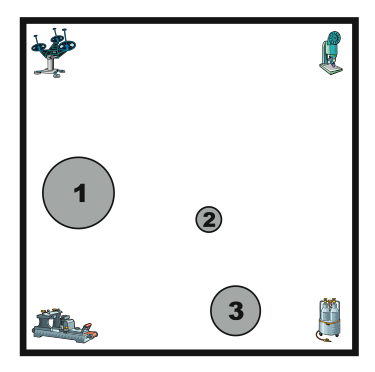
\includegraphics[width=0.7\textwidth]{fabriksrobot.png}
\caption{Explanation of the example. The critical distance is between pillars 1 and 2 in the input. The distance between their center points is approximately 405.123, and the actual distance between them is 405.12 - 110 - 30 = 265.12, making the maximum radius of the robot 265.12/2 = 132.56.}
\label{overflow}
\end{figure}

On a large factory floor (size $1000 \times 1000$ meters) there are a number of circular pillars with varying radii. The pillars do not touch each other or the walls. The company that owns the factory is planning to purchase a guard robot that will move around the premises. In the four corners of the premises there are machines that the robot must be able to reach by zigzagging between pillars and walls. The guard robots available on the market are all, like the pillars, completely circular. Before the company purchases a robot, however, they want to know the maximum radius the robot can have while still meeting their requirements.

No part of the robot may extend outside the premises. If the robot has radius $r$, it must be able to reach the points $(r, r)$, $(1000 - r, r)$, $(r, 1000 - r)$, and $(1000 - r, 1000 - r)$ to service the four machines from there. The machines never obstruct the robot's movement.

\section*{Input}
The first line contains an integer $n$ ($1 \le n \le 50$), the number of pillars in the premises.

Then follow $n$ lines, each containing 3 integers, $x$, $y$, and $r$. These numbers describe the coordinates of a pillar's center and its radius.


\section*{Output}
Output a floating-point number: the maximum radius of the robot. The answer is accepted if the difference between it and the judge's answer is less than $0.01$.

\section*{Scoring}
Your solution will be tested on a set of test groups.
To earn points for a group, you must pass all test cases in that group.

\noindent
\begin{tabular}{| l | l | p{12cm} |}
  \hline
  \textbf{Group} & \textbf{Points} & \textbf{Constraints} \\ \hline
  $1$    & $20$       & $n = 1$ \\ \hline
  $2$    & $80$       & No additional constraints. \\ \hline
\end{tabular}
